\documentclass{standalone}
\usepackage{pgfplots}
\usepackage{glossaries}

\newglossaryentry{pcnc}{
    name={PcNc},
    description={Some description}
}

\begin{document}
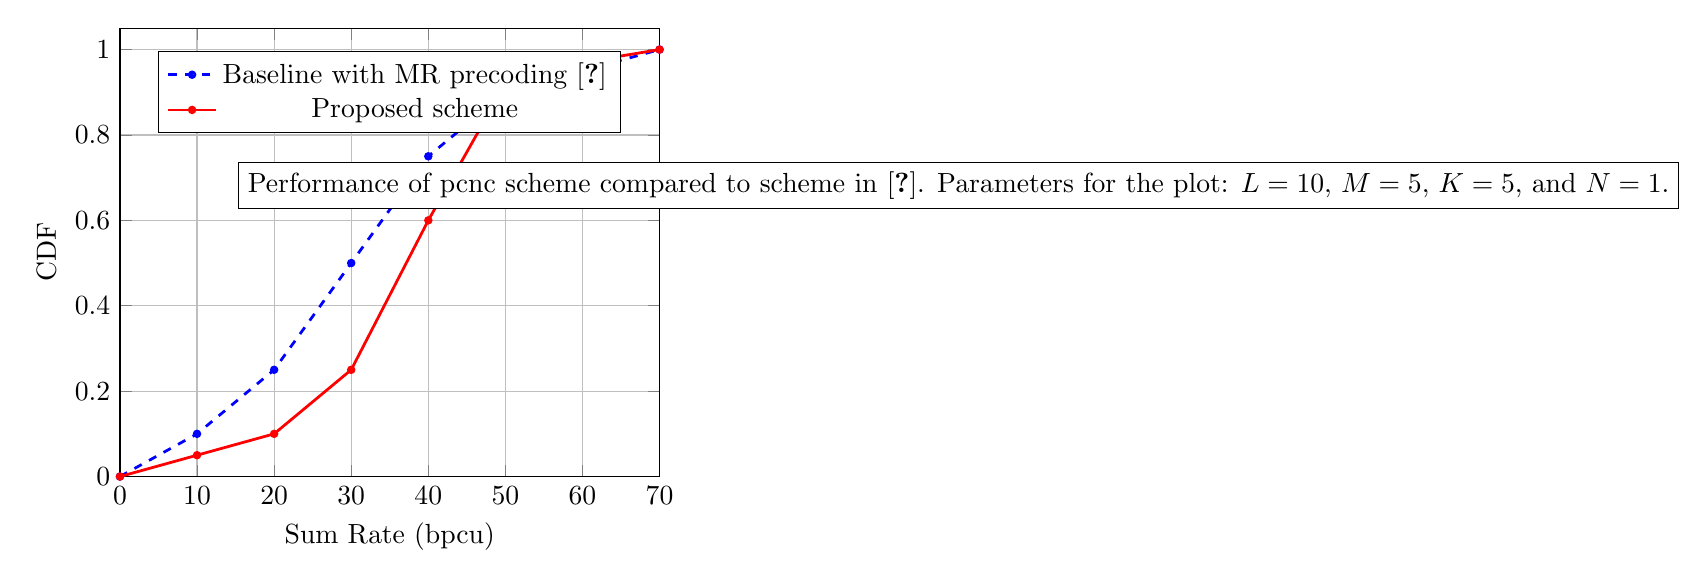
\begin{tikzpicture}
    \begin{axis}[
        xlabel={Sum Rate (bpcu)},
        ylabel={CDF},
        xmin=0, xmax=70,
        ymin=0, ymax=1.05,
        legend style={at={(0.5,0.95)}, anchor=north},
        grid=both,
        mark size=1pt
    ]
    % Baseline with MR precoding
    \addplot[
        color=blue,
        dashed,
        line width=1pt,
        mark=o,
        mark options={solid},
    ]
    coordinates {
        (0, 0)
        (10, 0.1)
        (20, 0.25)
        (30, 0.5)
        (40, 0.75)
        (50, 0.9)
        (60, 0.95)
        (70, 1)
    };
    
    % Proposed scheme
    \addplot[
        color=red,
        solid,
        line width=1pt,
        mark=*,
        mark options={solid},
    ]
    coordinates {
        (0, 0)
        (10, 0.05)
        (20, 0.1)
        (30, 0.25)
        (40, 0.6)
        (50, 0.92)
        (60, 0.97)
        (70, 1)
    };
    
    % Legend
    \legend{Baseline with MR precoding~\cite{antonioli2023mixed}, Proposed scheme}
    \end{axis}
    
    % Custom legend symbol description can be added if needed
    \node[draw,fill=white,anchor=north west] at (1.5,4) {Performance of \gls{pcnc} scheme compared to scheme in~\cite{antonioli2023mixed}. Parameters for the plot: $L=10$, $M=5$, $K=5$, and $N=1$.};
\end{tikzpicture}

% The following is just for handling \cite if needed in actual document
% \begin{thebibliography}{9}
%     \bibitem{antonioli2023mixed}
%     Author(s): Some Name(s), Title, Journal/Conference, Year.
% \end{thebibliography}
\end{document}